% Options for packages loaded elsewhere
\PassOptionsToPackage{unicode}{hyperref}
\PassOptionsToPackage{hyphens}{url}
\PassOptionsToPackage{dvipsnames,svgnames,x11names}{xcolor}
%
\documentclass[
  10pt,
  ignorenonframetext,
]{beamer}
\usepackage{pgfpages}
\setbeamertemplate{caption}[numbered]
\setbeamertemplate{caption label separator}{: }
\setbeamercolor{caption name}{fg=normal text.fg}
\beamertemplatenavigationsymbolsempty
% Prevent slide breaks in the middle of a paragraph
\widowpenalties 1 10000
\raggedbottom
\setbeamertemplate{part page}{
  \centering
  \begin{beamercolorbox}[sep=16pt,center]{part title}
    \usebeamerfont{part title}\insertpart\par
  \end{beamercolorbox}
}
\setbeamertemplate{section page}{
  \centering
  \begin{beamercolorbox}[sep=12pt,center]{part title}
    \usebeamerfont{section title}\insertsection\par
  \end{beamercolorbox}
}
\setbeamertemplate{subsection page}{
  \centering
  \begin{beamercolorbox}[sep=8pt,center]{part title}
    \usebeamerfont{subsection title}\insertsubsection\par
  \end{beamercolorbox}
}
\AtBeginPart{
  \frame{\partpage}
}
\AtBeginSection{
  \ifbibliography
  \else
    \frame{\sectionpage}
  \fi
}
\AtBeginSubsection{
  \frame{\subsectionpage}
}
\usepackage{amsmath,amssymb}
\usepackage{lmodern}
\usepackage{iftex}
\ifPDFTeX
  \usepackage[T1]{fontenc}
  \usepackage[utf8]{inputenc}
  \usepackage{textcomp} % provide euro and other symbols
\else % if luatex or xetex
  \usepackage{unicode-math}
  \defaultfontfeatures{Scale=MatchLowercase}
  \defaultfontfeatures[\rmfamily]{Ligatures=TeX,Scale=1}
\fi
\usetheme[]{Singapore}
\usefonttheme{serif}
% Use upquote if available, for straight quotes in verbatim environments
\IfFileExists{upquote.sty}{\usepackage{upquote}}{}
\IfFileExists{microtype.sty}{% use microtype if available
  \usepackage[]{microtype}
  \UseMicrotypeSet[protrusion]{basicmath} % disable protrusion for tt fonts
}{}
\makeatletter
\@ifundefined{KOMAClassName}{% if non-KOMA class
  \IfFileExists{parskip.sty}{%
    \usepackage{parskip}
  }{% else
    \setlength{\parindent}{0pt}
    \setlength{\parskip}{6pt plus 2pt minus 1pt}}
}{% if KOMA class
  \KOMAoptions{parskip=half}}
\makeatother
\usepackage{xcolor}
\newif\ifbibliography
\usepackage{color}
\usepackage{fancyvrb}
\newcommand{\VerbBar}{|}
\newcommand{\VERB}{\Verb[commandchars=\\\{\}]}
\DefineVerbatimEnvironment{Highlighting}{Verbatim}{commandchars=\\\{\}}
% Add ',fontsize=\small' for more characters per line
\usepackage{framed}
\definecolor{shadecolor}{RGB}{248,248,248}
\newenvironment{Shaded}{\begin{snugshade}}{\end{snugshade}}
\newcommand{\AlertTok}[1]{\textcolor[rgb]{0.94,0.16,0.16}{#1}}
\newcommand{\AnnotationTok}[1]{\textcolor[rgb]{0.56,0.35,0.01}{\textbf{\textit{#1}}}}
\newcommand{\AttributeTok}[1]{\textcolor[rgb]{0.77,0.63,0.00}{#1}}
\newcommand{\BaseNTok}[1]{\textcolor[rgb]{0.00,0.00,0.81}{#1}}
\newcommand{\BuiltInTok}[1]{#1}
\newcommand{\CharTok}[1]{\textcolor[rgb]{0.31,0.60,0.02}{#1}}
\newcommand{\CommentTok}[1]{\textcolor[rgb]{0.56,0.35,0.01}{\textit{#1}}}
\newcommand{\CommentVarTok}[1]{\textcolor[rgb]{0.56,0.35,0.01}{\textbf{\textit{#1}}}}
\newcommand{\ConstantTok}[1]{\textcolor[rgb]{0.00,0.00,0.00}{#1}}
\newcommand{\ControlFlowTok}[1]{\textcolor[rgb]{0.13,0.29,0.53}{\textbf{#1}}}
\newcommand{\DataTypeTok}[1]{\textcolor[rgb]{0.13,0.29,0.53}{#1}}
\newcommand{\DecValTok}[1]{\textcolor[rgb]{0.00,0.00,0.81}{#1}}
\newcommand{\DocumentationTok}[1]{\textcolor[rgb]{0.56,0.35,0.01}{\textbf{\textit{#1}}}}
\newcommand{\ErrorTok}[1]{\textcolor[rgb]{0.64,0.00,0.00}{\textbf{#1}}}
\newcommand{\ExtensionTok}[1]{#1}
\newcommand{\FloatTok}[1]{\textcolor[rgb]{0.00,0.00,0.81}{#1}}
\newcommand{\FunctionTok}[1]{\textcolor[rgb]{0.00,0.00,0.00}{#1}}
\newcommand{\ImportTok}[1]{#1}
\newcommand{\InformationTok}[1]{\textcolor[rgb]{0.56,0.35,0.01}{\textbf{\textit{#1}}}}
\newcommand{\KeywordTok}[1]{\textcolor[rgb]{0.13,0.29,0.53}{\textbf{#1}}}
\newcommand{\NormalTok}[1]{#1}
\newcommand{\OperatorTok}[1]{\textcolor[rgb]{0.81,0.36,0.00}{\textbf{#1}}}
\newcommand{\OtherTok}[1]{\textcolor[rgb]{0.56,0.35,0.01}{#1}}
\newcommand{\PreprocessorTok}[1]{\textcolor[rgb]{0.56,0.35,0.01}{\textit{#1}}}
\newcommand{\RegionMarkerTok}[1]{#1}
\newcommand{\SpecialCharTok}[1]{\textcolor[rgb]{0.00,0.00,0.00}{#1}}
\newcommand{\SpecialStringTok}[1]{\textcolor[rgb]{0.31,0.60,0.02}{#1}}
\newcommand{\StringTok}[1]{\textcolor[rgb]{0.31,0.60,0.02}{#1}}
\newcommand{\VariableTok}[1]{\textcolor[rgb]{0.00,0.00,0.00}{#1}}
\newcommand{\VerbatimStringTok}[1]{\textcolor[rgb]{0.31,0.60,0.02}{#1}}
\newcommand{\WarningTok}[1]{\textcolor[rgb]{0.56,0.35,0.01}{\textbf{\textit{#1}}}}
\usepackage{longtable,booktabs,array}
\usepackage{calc} % for calculating minipage widths
\usepackage{caption}
% Make caption package work with longtable
\makeatletter
\def\fnum@table{\tablename~\thetable}
\makeatother
\usepackage{graphicx}
\makeatletter
\def\maxwidth{\ifdim\Gin@nat@width>\linewidth\linewidth\else\Gin@nat@width\fi}
\def\maxheight{\ifdim\Gin@nat@height>\textheight\textheight\else\Gin@nat@height\fi}
\makeatother
% Scale images if necessary, so that they will not overflow the page
% margins by default, and it is still possible to overwrite the defaults
% using explicit options in \includegraphics[width, height, ...]{}
\setkeys{Gin}{width=\maxwidth,height=\maxheight,keepaspectratio}
% Set default figure placement to htbp
\makeatletter
\def\fps@figure{htbp}
\makeatother
\setlength{\emergencystretch}{3em} % prevent overfull lines
\providecommand{\tightlist}{%
  \setlength{\itemsep}{0pt}\setlength{\parskip}{0pt}}
\setcounter{secnumdepth}{-\maxdimen} % remove section numbering
\newlength{\cslhangindent}
\setlength{\cslhangindent}{1.5em}
\newlength{\csllabelwidth}
\setlength{\csllabelwidth}{3em}
\newlength{\cslentryspacingunit} % times entry-spacing
\setlength{\cslentryspacingunit}{\parskip}
\newenvironment{CSLReferences}[2] % #1 hanging-ident, #2 entry spacing
 {% don't indent paragraphs
  \setlength{\parindent}{0pt}
  % turn on hanging indent if param 1 is 1
  \ifodd #1
  \let\oldpar\par
  \def\par{\hangindent=\cslhangindent\oldpar}
  \fi
  % set entry spacing
  \setlength{\parskip}{#2\cslentryspacingunit}
 }%
 {}
\usepackage{calc}
\newcommand{\CSLBlock}[1]{#1\hfill\break}
\newcommand{\CSLLeftMargin}[1]{\parbox[t]{\csllabelwidth}{#1}}
\newcommand{\CSLRightInline}[1]{\parbox[t]{\linewidth - \csllabelwidth}{#1}\break}
\newcommand{\CSLIndent}[1]{\hspace{\cslhangindent}#1}
\ifLuaTeX
  \usepackage{selnolig}  % disable illegal ligatures
\fi
\IfFileExists{bookmark.sty}{\usepackage{bookmark}}{\usepackage{hyperref}}
\IfFileExists{xurl.sty}{\usepackage{xurl}}{} % add URL line breaks if available
\urlstyle{same} % disable monospaced font for URLs
\hypersetup{
  pdftitle={Module 11: Deep Learning and Neural Networks},
  pdfauthor={Stefanie Muff, Department of Mathematical Sciences, NTNU},
  colorlinks=true,
  linkcolor={Maroon},
  filecolor={Maroon},
  citecolor={Blue},
  urlcolor={blue},
  pdfcreator={LaTeX via pandoc}}

\title{Module 11: Deep Learning and Neural Networks}
\subtitle{TMA4268 Statistical Learning V2023}
\author{Stefanie Muff, Department of Mathematical Sciences, NTNU}
\date{April 24 and 27, 2023}

\begin{document}
\frame{\titlepage}

\begin{frame}{Acknowledgements}
\protect\hypertarget{acknowledgements}{}
\(~\)

\begin{itemize}
\item
  Some of this material was (in a modified version) created by Mette
  Langaas who has put a lot of effort in creating this module in its
  original version. Thanks to Mette for the permission to use the
  material!
\item
  Some of the figures and slides in this presentation are taken (or are
  inspired) from James et al. (2021).
\end{itemize}
\end{frame}

\begin{frame}
\begin{block}{Learning material for this module}
\protect\hypertarget{learning-material-for-this-module}{}
\vspace{2mm}

\begin{itemize}
\item
  James et al (2021): An Introduction to Statistical Learning. Chapter
  10.
\item
  All the material presented on these module slides and in class.
\item
  Videos on neural networsk and back propagation

  \begin{itemize}
  \tightlist
  \item
    \href{https://www.youtube.com/watch?v=aircAruvnKk}{Video 1}
  \item
    \href{https://www.youtube.com/watch?v=IHZwWFHWa-w}{Video 2}
  \item
    \href{https://www.youtube.com/watch?v=Ilg3gGewQ5U}{Video 3}
  \item
    \href{https://www.youtube.com/watch?v=tIeHLnjs5U8}{Video 4}
  \end{itemize}
\end{itemize}

\(~\)

\textbf{Secondary material (not compulsory):}

\vspace{2mm}

\begin{itemize}
\tightlist
\item
  Background material: Chapters 6-8 Goodfellow, Bengio, and Courville
  (2016) \url{https://www.deeplearningbook.org}
\end{itemize}

\(~\)

See also \emph{References and further reading} (last slide), for further
reading material.
\end{block}
\end{frame}

\begin{frame}
\begin{block}{What will you learn?}
\protect\hypertarget{what-will-you-learn}{}
\(~\)

\begin{itemize}
\tightlist
\item
  Deep learning: The timeline
\end{itemize}

\vspace{2mm}

\begin{itemize}
\tightlist
\item
  Single and multilayer feed-forward networks
\end{itemize}

\vspace{2mm}

\begin{itemize}
\tightlist
\item
  Convolutional neural networks (CNNs)
\end{itemize}

\vspace{2mm}

\begin{itemize}
\tightlist
\item
  Recurrent neural networks (RNNs)
\end{itemize}

\vspace{2mm}

\begin{itemize}
\tightlist
\item
  When to use deep learning?
\end{itemize}
\end{block}
\end{frame}

\begin{frame}{Introduction: Time line}
\protect\hypertarget{introduction-time-line}{}
\(~\)

\begin{itemize}
\item
  1950's: First neural networks (NN) in ``toy form''.
\item
  1980s: the backpropagation algorithm was rediscovered.
\item
  1989: (Bell Labs, Yann LeCun) used convolutional neural networks to
  classifying handwritten digits.
\item
  2000s: After the first hype, NNs were pushed aside by boosting and
  support vector machines in the 2000s.
\item
  Since 2010: Revival! The emergence of \emph{Deep learning} as a
  consequence of improved computer resources, some innovations, and
  applications to image and video classification, and speech and text
  processing.
\end{itemize}

\(~\)
\end{frame}

\begin{frame}
\begin{itemize}
\tightlist
\item
  Shift from statistics to computer science and machine learning, as
  they are highly parameterized.
\end{itemize}

\(~\)

\begin{itemize}
\tightlist
\item
  Statisticians were skeptical: ``It's just a nonlinear model''.
\end{itemize}
\end{frame}

\begin{frame}
\centering

\includegraphics[width=0.5\textwidth,height=\textheight]{Neuron3.png}

\flushleft

Neuron and myelinated axon, with signal flow from inputs at dendrites to
outputs at axon terminals.

\scriptsize

Image credits: By Egm4313.s12 (Prof.~Loc Vu-Quoc)
\url{https://commons.wikimedia.org/w/index.php?curid=72816083}
\end{frame}

\begin{frame}
\begin{itemize}
\tightlist
\item
  There are several learning resources (some listed under `further
  references') that you my turn to for further knowledge into deep
  learning.
\item
  There is a new IT3030
  \href{https://www.ntnu.no/studier/emner/IT3030\#tab=omEmnet}{deep
  learning course at NTNU}.
\end{itemize}

\centering

\includegraphics[width=0.3\textwidth,height=\textheight]{DeepLearningwithR.jpeg}
\includegraphics[width=0.3\textwidth,height=\textheight]{DeepLearning.jpeg}
\end{frame}

\begin{frame}
\begin{block}{AI, machine learning and statistics}
\protect\hypertarget{ai-machine-learning-and-statistics}{}
\includegraphics[angle=-90]{AI_ML_DL.png}
\end{block}
\end{frame}

\begin{frame}
\begin{block}{AI}
\protect\hypertarget{ai}{}
\(~\)

\begin{itemize}
\tightlist
\item
  Artificial intelligence (AI) dates back to the 1950s, and can be seen
  as \emph{the effort to automate intellectual tasks normally performed
  by humans} (page 4, Chollet and Allaire (2018)).
\end{itemize}

\(~\)

\begin{itemize}
\tightlist
\item
  AI was first based on hardcoded rules (like in chess programs), but
  turned out to be intractable for solving more complex, fuzzy problems.
\end{itemize}

\(~\)
\end{block}
\end{frame}

\begin{frame}
\begin{block}{Machine learning}
\protect\hypertarget{machine-learning}{}
\(~\)

\begin{itemize}
\tightlist
\item
  With the field of \emph{machine learning} the shift is that a system
  is \emph{trained} rather than explicitly programmed.
\end{itemize}

\(~\)

\begin{itemize}
\tightlist
\item
  ML deals with much larger and more complex data sets than what is
  usually done in statistics.
\end{itemize}

\(~\)

\begin{itemize}
\tightlist
\item
  The focus in ML is oriented towards \emph{engineering}, and ideas are
  proven \emph{empirically} rather than theoretically (which is the case
  in mathematical statistics).
\end{itemize}

\(~\)

According to Chollet and Allaire (2018) (page 19): \vspace{2mm}

\emph{Machine learning isn't mathematics or physics, {[}\ldots{]} it's
an engineering science.}
\end{block}
\end{frame}

\begin{frame}
\begin{block}{Deep learning}
\protect\hypertarget{deep-learning}{}
\(~\)

\begin{quote}
Deep Learning is an algorithm which has no theoretical limitations of what it can learn; the more data you give and the more computational time you provide, the better it is. 

Geoffrey Hinton (Google)
\end{quote}

\(~\)

\begin{itemize}
\tightlist
\item
  \emph{Deep} does not refer to a deeper understanding.
\end{itemize}

\(~\)

\begin{itemize}
\tightlist
\item
  Rather, deep referes to the \emph{layers of representation}, for
  example in a neural network.
\end{itemize}

\(~\)

\center

\includegraphics[width=0.8\textwidth,height=\textheight]{deep.png}
\end{block}
\end{frame}

\begin{frame}
\begin{itemize}
\tightlist
\item
  In 2011 neural networks with many layers were performing well on image
  classification tasks.
\end{itemize}

\vspace{2mm}

\begin{itemize}
\tightlist
\item
  The \href{http://www.image-net.org/}{\emph{ImageNet}} classification
  challenge (classify high resolution colour images into 1k different
  categories after training on 1.4M images) was won by solutions with
  deep convolutional neural networks (CNNs). In 2011 the accuracy was
  74.3\%, in 2012 83.6\% and in 2015 96.4\%.
\end{itemize}

\vspace{2mm}

\begin{itemize}
\tightlist
\item
  Since 2012, CNNs are the general solution for computer vision tasks.
  Other application area: natural language processing.
\end{itemize}
\end{frame}

\begin{frame}
The success of deep learning is dependent upon the breakthroughts in

\begin{itemize}
\tightlist
\item
  \emph{hardware} development, expecially with faster CPUs and massively
  parallell graphical processing units (GPUs).
\item
  \emph{datasets} and benchmarks (internet/tech data).
\item
  improvemets of the \emph{algorithms}.
\end{itemize}

\(~\)

Achievements of deep learning includes

\begin{itemize}
\tightlist
\item
  high quality (near-human to super human) image classification,
\item
  speech recognition,
\item
  handwriting transcription,
\item
  autonomous driving, and more!
\end{itemize}
\end{frame}

\begin{frame}{Feedforward networks}
\protect\hypertarget{feedforward-networks}{}
\centering

\includegraphics[width=0.8\textwidth,height=\textheight]{drawNNp3h2o3.png}
\end{frame}

\begin{frame}
\begin{block}{The single hidden layer feedforward network}
\protect\hypertarget{the-single-hidden-layer-feedforward-network}{}
\(~\)

The nodes are also called \emph{neurons}.

\(~\)

\textbf{Notation}

\(~\)

\begin{enumerate}
\tightlist
\item
  Inputs: \(p\) input layer nodes
  \({\boldsymbol{x}^\top} = (x_1, x_2, \ldots, x_p)\).
\item
  The nodes \(z_m\) in the hidden layer, \(m=1,\ldots, M\); as vector
  \({\boldsymbol z}^\top=(z_1, \ldots, z_M)\), and the hidden layer
  activation function \(g()\). \[
  z_m({\boldsymbol x})=g(\alpha_{0m}+\sum_{j=1}^p \alpha_{jm}x_{j})
  \] where \(\alpha_{jm}\) is the
  weight\footnote{We stick with greek letters $\alpha$ and $\beta$ for parameters, but call them weights.}
  from input \(j\) to hidden node \(m\), and \(\alpha_{0m}\) is the bias
  term for the \(m\)th hidden node.
\end{enumerate}
\end{block}
\end{frame}

\begin{frame}
\begin{enumerate}
\setcounter{enumi}{2}
\tightlist
\item
  The node(s) in the output layer, \(c=1,\ldots C\):
  \(y_1, y_2, \ldots, y_C\), or as vector \({\boldsymbol y}\), and
  output layer activation function \(f()\). \[
  \hat{y}_c({\boldsymbol x})=f(\beta_{0c}+\sum_{m=1}^M \beta_{mc}z_{m}({\boldsymbol x}))
  \] where \(\beta_{mc}\) is from hidden neuron \(m\) to ouput node
  \(c\), and \(\beta_{0c}\) is the bias term for the \(c\)th output
  node.
\end{enumerate}

\(~\)

\begin{enumerate}
\setcounter{enumi}{3}
\tightlist
\item
  Taken together \[
  \hat{y}_c({\boldsymbol x})=f(\beta_{0c}+\sum_{m=1}^M \beta_{mc}z_{m})=f(\beta_{0c}+\sum_{m=1}^M \beta_{mc}g(\alpha_{0m}+\sum_{j=1}^p \alpha_{jm}x_{j}))
  \]
\end{enumerate}
\end{frame}

\begin{frame}
\textbf{Hands on:}

\(~\)

\begin{itemize}
\tightlist
\item
  Identify \(p, M, C\) in the network figure above, and relate that to
  the \(y_{c}({\boldsymbol x})\) equation.
\end{itemize}

\(~\)

\begin{itemize}
\tightlist
\item
  How many parameters (the \(\alpha\) and \(\beta\)s) need to be
  estimated for this network?
\end{itemize}

\(~\)

\begin{itemize}
\tightlist
\item
  What determines the values of \(p\) and \(C\)?
\end{itemize}

\(~\)

\begin{itemize}
\tightlist
\item
  How is \(M\) determined?
\end{itemize}
\end{frame}

\begin{frame}
\begin{block}{Special case: linear activation function for the hidden
layer}
\protect\hypertarget{special-case-linear-activation-function-for-the-hidden-layer}{}
\(~\)

If we assume that \(g(z)=z\) (linear or identity activiation):

\[
\hat{y}_c({\boldsymbol x})= f(\beta_{0c}+\sum_{m=1}^M \beta_{mc}(\alpha_{0m}+\sum_{j=1}^p \alpha_{jm}x_{j}))
\]

\(~\) \(~\)

\textbf{Q:} Does this look like something you have seen before?

\(~\)

\textbf{A:}
\end{block}
\end{frame}

\begin{frame}
\begin{block}{Multilayer neural networks}
\protect\hypertarget{multilayer-neural-networks}{}
\(~\)

Alternative: networks with more than one hidden layer. A network with
\emph{many hidden layers} is called a \emph{deep network}.

\centering

\includegraphics[width=0.7\textwidth,height=\textheight]{fig10_4.png}

\scriptsize

(Fig 10.4 James et al. (2021))
\end{block}
\end{frame}

\begin{frame}
\begin{itemize}
\tightlist
\item
  The idea of the multilayer NN is exactly the same as for the
  single-layer version.
\end{itemize}

\(~\)

\begin{itemize}
\tightlist
\item
  \(f_m(X)\) is a (transformation of) the linear combination of the last
  layer.
\end{itemize}
\end{frame}

\begin{frame}
\begin{block}{Outcome encoding}
\protect\hypertarget{outcome-encoding}{}
\(~\)

\begin{itemize}
\tightlist
\item
  \emph{Continuous} and \emph{binary} may only have one output node
  (\(y_i=\) observed value).
\end{itemize}

\(~\)

\begin{itemize}
\tightlist
\item
  For \(C\) \emph{categories}, we have \(C\) output nodes, where we
  encode the output as \(Y = (Y_1, Y_2, \ldots, Y_C)\) , where
  \({\boldsymbol y}_i=(0,0,\ldots,0,1,0,\ldots,0)\) with a value of
  \(1\) in the \(c^{th}\) element of \({\boldsymbol y}_i\) if the class
  is \(c\). This is called \emph{\textcolor{red}{one-hot encoding}} or
  \emph{dummy encoding}.
\end{itemize}

\(~\)
\end{block}
\end{frame}

\begin{frame}
\begin{block}{Example: MNIST dataset}
\protect\hypertarget{example-mnist-dataset}{}
\(~\)

\begin{itemize}
\tightlist
\item
  Aim: Classification of handwritten digits.
\end{itemize}

\(~\)

\begin{itemize}
\tightlist
\item
  Categorical outcome \(C=0,1,\ldots,9\).
\end{itemize}

\(~\)

\begin{itemize}
\tightlist
\item
  This data has been analysed with a single-layer feed-forward network
  in a previous version of the course:
  \url{https://www.math.ntnu.no/emner/TMA4268/2018v/11NN/8-neural_networks_mnist.html}.
\end{itemize}
\end{block}
\end{frame}

\begin{frame}
Objective: classify the digit contained in an image (28 \(\times\) 28
greyscale).

\includegraphics{mnist.png}
\end{frame}

\begin{frame}
\begin{block}{Neural network parts}
\protect\hypertarget{neural-network-parts}{}
\(~\)

We now focus on the different elements of neural networks.

\(~\)

\begin{enumerate}
[1)]
\tightlist
\item
  Output layer activation
\end{enumerate}

\vspace{2mm}

\begin{enumerate}
[1)]
\setcounter{enumi}{1}
\tightlist
\item
  Hidden layer activation
\end{enumerate}

\vspace{2mm}

\begin{enumerate}
[1)]
\setcounter{enumi}{2}
\tightlist
\item
  Network architecture
\end{enumerate}

\vspace{2mm}

\begin{enumerate}
[1)]
\setcounter{enumi}{3}
\tightlist
\item
  Loss function
\end{enumerate}

\vspace{2mm}

\begin{enumerate}
[1)]
\setcounter{enumi}{4}
\tightlist
\item
  Optimizers
\end{enumerate}
\end{block}
\end{frame}

\begin{frame}
\begin{block}{1) Output layer activation}
\protect\hypertarget{output-layer-activation}{}
\(~\)

These choices have been guided by solutions in statistics (multiple
linear regression, logistic regression, multiclass regression)

\(~\)

\begin{itemize}
\item
  \emph{\textcolor{red}{Linear activation}}: for \emph{continuous
  outcome} (regression problems) \[f(X)=X \ .\]
\item
  \emph{\textcolor{red}{Sigmoid activation}}: for \emph{binary outcome}
  (two-class classification problems)
  \[f(X)=\text{Pr}(Y=1 | X ) = \frac{1}{1+\exp(-X)} = \frac{\exp(X)}{1+\exp(X)} \ .\]
\item
  \emph{\textcolor{red}{Softmax}}: for \emph{multinomial/categorical
  outcome} (multi-class classification problems) \[
  f_m(X) =  \text{Pr}(Y=m | X ) = \frac{\exp(Z_m)}{\sum_{s=1}^{C}\exp(Z_s)} \ .
  \]
\end{itemize}

\scriptsize

Note that we denote by \(Z_m\) the value in the output node \(m\)
\emph{before} the output layer activation.
\end{block}
\end{frame}

\begin{frame}
\begin{block}{2) Hidden layer activation}
\protect\hypertarget{hidden-layer-activation}{}
\tiny

(See chapter 6.3 in Goodfellow, Bengio, and Courville (2016))

\normalsize

\(~\)

\textbf{Very common}:

\(~\)

\begin{itemize}
\tightlist
\item
  The \textbf{sigmoid} \(g=\sigma(x)=1/(1+\exp(-x))\) (logistic)
  activation functions.
\item
  The \textbf{rectified linear unit (ReLU)} \(g(x)=\max(0,x)\)
  activation functions.
\end{itemize}

\vspace{2mm}

\centering

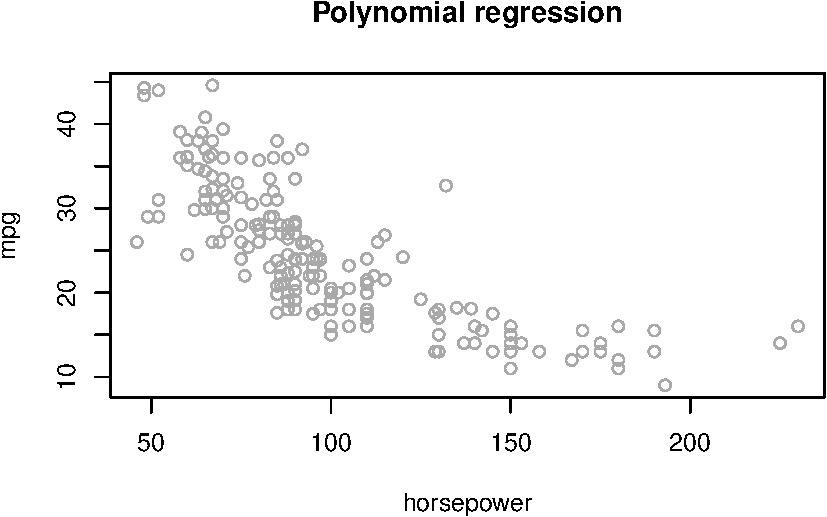
\includegraphics[width=0.8\linewidth]{11Nnet_files/figure-beamer/unnamed-chunk-1-1}
\end{block}
\end{frame}

\begin{frame}
\textbf{Less common}:

\(~\)

\begin{itemize}
\tightlist
\item
  Radial basis functions: as we looked at in Module 9.
\end{itemize}

\(~\)

\begin{itemize}
\tightlist
\item
  Softplus: \(g(x)=\ln(1+\exp(x))\)
\end{itemize}

\(~\)

\begin{itemize}
\tightlist
\item
  Hard tanh: \(g(x)=\max(-1,\min(1,x))\)
\end{itemize}
\end{frame}

\begin{frame}
Among all the possibilities, ReLU is nowadays the most popular one. Why?

\(~\)

\begin{itemize}
\tightlist
\item
  The function is piecewise linear, but \emph{in total non-linear}.
\end{itemize}

\(~\)

\begin{itemize}
\tightlist
\item
  Replacing sigmoid with ReLU is reported to be one of the major changes
  that have improved the performance of the feedforward
  networks\footnote{Goodfellow et al, Section 6.6}.
\end{itemize}
\end{frame}

\begin{frame}
\begin{block}{Universal approximation property}
\protect\hypertarget{universal-approximation-property}{}
\(~\)

\begin{itemize}
\tightlist
\item
  Think of the goal of a feedforward network to approximate some
  function \(f\), mapping our input vector \({\boldsymbol x}\) to an
  output value \({\boldsymbol y}\).
\end{itemize}

\(~\)

\begin{itemize}
\tightlist
\item
  What type of mathematical function can a feedforward neural network
  with one hidden layer and linear output activation represent?
\end{itemize}

\(~\) \pause

The \emph{universal approximation
theorem}\footnote{Goodfellow et al 2016, Section 6.4.1, https://www.deeplearningbook.org}
says that a feedforward network with \vspace{2mm}

\begin{itemize}
\tightlist
\item
  a \emph{linear output layer}
\item
  at least one hidden layer with a ``squashing'' activation function
  (e.g., ReLU or sigmoid) and ``enough'' hidden units
\end{itemize}

\vspace{2mm}

can approximate any (Borel measurable) function from one
finite-dimensional space (our input layer) to another (our output layer)
with any desired non-zero amount of error.
\end{block}
\end{frame}

\begin{frame}
\begin{block}{3) Network architecture}
\protect\hypertarget{network-architecture}{}
\(~\)

Network architecture contains three components:

\(~\)

\begin{itemize}
\item
  \emph{Width}: How many nodes are in each layer of the network?
\item
  \emph{Depth}: How deep is the network (how many hidden layers)?
\item
  \emph{Connectivity}: How are the nodes connected to each other?
\end{itemize}

\(~\)

Especially the connectivity depends on the problem, and here experience
is important.

\(~\)

\begin{itemize}
\tightlist
\item
  We will consider \emph{feedforward networks}, \emph{convolutional
  neural networks (CNNs)} and \emph{recursive neural networks (RNNs)}.
\end{itemize}
\end{block}
\end{frame}

\begin{frame}
However, the recent practice is to

\(~\)

\begin{itemize}
\tightlist
\item
  choose a too large network, train it until convergence (optimum),
  which results in overfitting,
\end{itemize}

\vspace{2mm}

\begin{itemize}
\tightlist
\item
  then use other means to avoid this (various variants of regularization
  and hyperparameter optimization).
\end{itemize}

\(~\)

This simplifies the choice of network architecture to \emph{choose a
large enough network}.

\(~\)

See e.g. Chollet and Allaire (2018), Section 4.5.6/7 and Goodfellow,
Bengio, and Courville (2016), Section 7
\end{frame}

\begin{frame}[fragile]
\begin{block}{4) Loss function (``Method'')}
\protect\hypertarget{loss-function-method}{}
\(~\)

\begin{itemize}
\tightlist
\item
  The choice of the loss function is closely related to the output layer
  activation function.
\end{itemize}

\(~\)

\begin{itemize}
\tightlist
\item
  Most popular problem types, output activation and loss functions:
\end{itemize}

\scriptsize

\begin{longtable}[]{@{}llll@{}}
\toprule()
Problem & Output nodes & Output activation & Loss function \\
\midrule()
\endhead
Regression & 1 & \texttt{linear} & \texttt{mse} \\
Classification (C=2) & 1 & \texttt{sigmoid} &
\texttt{binary\_crossentropy} \\
Classification (C\textgreater2) & C & \texttt{softmax} &
\texttt{categorical\_crossentropy} \\
\bottomrule()
\end{longtable}
\end{block}
\end{frame}

\begin{frame}
\begin{itemize}
\tightlist
\item
  Regression: Loss function \emph{\textcolor{red}{MSE}} for a given set
  of parameters \(\boldsymbol{\theta}\):
\end{itemize}

\[J({\boldsymbol \theta}) = \sum_{i=1}^n (y_i- f(x_i))^2\]

\(~\)

\begin{itemize}
\tightlist
\item
  Classification: \emph{\textcolor{red}{Cross-entropy}}
\end{itemize}

\[J({\boldsymbol \theta}) = -\sum_{i=1}^n \sum_{m=1}^C y_i \log f_m(x_i) \ ,\]

\begin{itemize}
\tightlist
\item
  with special case for \(C=2\)
  (\emph{\textcolor{red}{binary cross-entropy loss}}):
  \[J({\boldsymbol \theta}) = -\sum_{i=1}^n  y_i \log f_m(x_i) + (1-y_i) \log (1-f_m(x_i)) \ .\]
\end{itemize}
\end{frame}

\begin{frame}
\begin{block}{5) Optimizors}
\protect\hypertarget{optimizors}{}
\(~\)

Let the unknown parameters be denoted \({\boldsymbol \theta}\) (what we
have previously denoted as \(\alpha\)s and \(\beta\)s), and the loss
function to be minimized \(J({\boldsymbol \theta})\).

\(~\)

\begin{itemize}
\item
  Gradient descent
\item
  Mini-batch stochastic gradient descent (SGD) and true SGD
\item
  Backpropagation
\end{itemize}
\end{block}
\end{frame}

\begin{frame}
\begin{block}{Gradient descent}
\protect\hypertarget{gradient-descent}{}
\(~\)

\begin{itemize}
\tightlist
\item
  We minimize a \emph{cost function} by iteratively tweaking the
  parameters along the negative gradient.
\end{itemize}

\(~\)

\center

\includegraphics[width=0.6\textwidth,height=\textheight]{gradient_descent.png}

\tiny (\url{https://github.com/SoojungHong/MachineLearning/wiki/Gradient-Descent})

\(~\)

\(~\)

\normalsize
\flushleft

\begin{itemize}
\tightlist
\item
  In practice this happens in a \emph{high-dimensional} parameters
  space, along the partial derivatives for each parameter.
\end{itemize}
\end{block}
\end{frame}

\begin{frame}
\begin{block}{Finding optimal weights: Gradient descent algorithm}
\protect\hypertarget{finding-optimal-weights-gradient-descent-algorithm}{}
\vspace{2mm}

\begin{enumerate}
\tightlist
\item
  Let \(t=0\) and denote the given initial values for the parameters
  \({\boldsymbol \theta}^{(t)}\). \vspace{2mm}
\item
  Until finding a (local) optimum, repeat a) to e)

  \begin{enumerate}
  [a)]
  \tightlist
  \item
    Calculate the predictions \({\hat{y}_1({\boldsymbol x}_i)}\).
  \item
    Calculate the loss function \(J({\boldsymbol \theta}^{(t)})\).
  \item
    Find the gradient (direction) in the \((p+1)\)-dimensional space of
    the weights, and evaluate this at the current weight values
    \(\nabla J({\boldsymbol \theta}^{(t)})={\frac{\partial J}{\partial {\boldsymbol \theta}}}({\boldsymbol \theta}^{(t)})\).
  \item
    Go with a given step length (\emph{\textcolor{red}{learning rate}})
    \(\lambda\) in the direction of the negative of the gradient of the
    loss function to get
    \[{\boldsymbol \theta}^{(t+1)}={\boldsymbol \theta}^{(t)} - \lambda \nabla J({\boldsymbol \theta}^{(t)}) \ .\]
  \item
    Set \(t=t+1\). \vspace{2mm}
  \end{enumerate}
\item
  The final values of the weights in that \((p+1)\) dimensional space
  are our parameter estimates and your network is \emph{trained}.
\end{enumerate}
\end{block}
\end{frame}

\begin{frame}
\textbf{Q}: Why are we moving in the direction of the negative of the
gradient? Why not the positive?

\textbf{A}:
\end{frame}

\begin{frame}
\begin{block}{Full vs.~stochastic gradient descent (SGD)}
\protect\hypertarget{full-vs.-stochastic-gradient-descent-sgd}{}
\(~\)

\begin{itemize}
\item
  Note that in \emph{full gradient descent}, the loss function is
  computed as a mean over all training examples. \[
  J({\boldsymbol \theta})=\frac{1}{n}\sum_{i=1}^n J({\boldsymbol x}_i, y_i) \ .
  \]
\item
  The gradient is \emph{an average over many individual gradients} from
  the training example. You can think of this as an estimator for an
  expectation.
\end{itemize}

\[
\nabla_{\boldsymbol \theta} J({\boldsymbol \theta})=\frac{1}{n}\sum_{i=1}^n \nabla_{\boldsymbol \theta} J({\boldsymbol x}_i, y_i) \ .
\]

\begin{itemize}
\tightlist
\item
  To build a network that generalizes well, it is important to have many
  training examples, but that would make us spend a lot of time and
  computer resources at calculating each gradient descent step.
\end{itemize}
\end{block}
\end{frame}

\begin{frame}
\begin{block}{Mini-batch stochastic gradient descent (SGD)}
\protect\hypertarget{mini-batch-stochastic-gradient-descent-sgd}{}
\(~\)

\textbf{Crucial idea}:

The expectation can be approximated by the average gradient over just a
\emph{\textcolor{red}{mini-batch}} (random sample) of the observations.

\(~\)

\textbf{Advantages}:

\vspace{1mm}

\begin{itemize}
\tightlist
\item
  The optimizer will converge much faster if it can rapidly compute
  approximate estimates of the gradient.
\end{itemize}

\vspace{1mm}

\begin{itemize}
\tightlist
\item
  Mini-batches may be processed \emph{in parallel}, and the batch size
  is often a power of 2 (32 or 256).
\end{itemize}

\vspace{1mm}

\begin{itemize}
\tightlist
\item
  Small batches also bring in a
  \emph{\textcolor{red}{regularization effect}}, maybe due to the
  variability they bring to the optimization process.
\end{itemize}
\end{block}
\end{frame}

\begin{frame}
\textbf{Mini-batch stochastic gradient descent}

\vspace{1mm}

\begin{enumerate}
\tightlist
\item
  Divide all the training samples randomly into \emph{mini-batches}.
\end{enumerate}

\vspace{1mm}

\begin{enumerate}
\setcounter{enumi}{1}
\tightlist
\item
  Until convergence, repeat a) to d)

  \begin{enumerate}
  [a)]
  \tightlist
  \item
    For each mini-batch: Make predictions of the reponses in the
    mini-batch in a \emph{forward pass}.
  \item
    Compute the loss for the training data in this batch.
  \item
    Compute the gradient
    \(\nabla_{\boldsymbol \theta}^* J({\boldsymbol \theta}^{(t)})\) of
    the loss with regard to the model's parameters (\emph{backward
    pass}) based on the training data in the batch.
  \item
    Update all weighs, but just using the \emph{average gradient} from
    the mini-batch
    \({\boldsymbol \theta}^{(t+1)}={\boldsymbol \theta}^{(t)} - \lambda \nabla_{\boldsymbol \theta} ^* J({\boldsymbol \theta}^{(t)})\)
  \end{enumerate}
\end{enumerate}

\vspace{1mm}

\begin{enumerate}
\setcounter{enumi}{2}
\tightlist
\item
  Network is \emph{trained}; return parameter estimates.
\end{enumerate}

\vspace{6mm}

\textbf{Special case}: \emph{\textcolor{red}{True SGD}} involves only
\emph{\textcolor{red}{one sample}} (mini-batch size 1). \(\rightarrow\)
Mini-batch SGD is a compromise between SGD (one sample per iteration)
and full gradient descent (full dataset per iteration)
\end{frame}

\begin{frame}
In the 3rd video (on backpropagation) from 3Blue1Brown there is nice
example of one trajectory from gradient decent and one from SGD (10:10
minutes into the video):
\url{https://www.youtube.com/watch?v=Ilg3gGewQ5U\&list=PLZHQObOWTQDNU6R1_67000Dx_ZCJB-3pi\&index=3}
\end{frame}

\begin{frame}
\begin{block}{Backpropagation algorithm}
\protect\hypertarget{backpropagation-algorithm}{}
\(~\)

\begin{itemize}
\tightlist
\item
  \emph{Backpropagation} is a simple and inexpensive way \emph{to
  calculate the gradient}.
\end{itemize}

\vspace{2mm}

\begin{itemize}
\tightlist
\item
  Computing the analytical expression for the gradient \(\nabla J\) is
  not difficult, but \emph{the numerical evaluation may be expensive}.
\end{itemize}

\vspace{2mm}

\vspace{2mm}

\begin{itemize}
\tightlist
\item
  The \emph{chain rule} is used to compute derivatives of functions of
  other functions where the derivatives are known. This is efficiently
  done with backpropagation.
\end{itemize}
\end{block}
\end{frame}

\begin{frame}
More background:

\(~\)

\begin{itemize}
\tightlist
\item
  James et al. (2021) Chapter 10.7.
\end{itemize}

\(~\)

\begin{itemize}
\tightlist
\item
  Mathematical details: Goodfellow, Bengio, and Courville (2016) Section
  6.5.\\
\end{itemize}

\(~\)

\begin{itemize}
\tightlist
\item
  3Blue1Brown videos: \url{https://www.youtube.com/watch?v=Ilg3gGewQ5U}
  and \url{https://www.youtube.com/watch?v=tIeHLnjs5U8}
\end{itemize}
\end{frame}

\begin{frame}
\begin{block}{Regularization}
\protect\hypertarget{regularization}{}
\(~\)

\begin{itemize}
\tightlist
\item
  Often: more weights than data samples \(\rightarrow\) danger for
  over-fitting.
\end{itemize}

\vspace{2mm}

\begin{itemize}
\tightlist
\item
  Regularization: \emph{any modification we make to a learning algorithm
  that is intended to reduce its generalization error but not its
  training error} \footnote{Goodfellow, Chapter 7}.
\end{itemize}

\vspace{2mm}

\begin{itemize}
\tightlist
\item
  Remember (module 6): The aim of regularization was to trade
  \emph{increased bias} for \emph{reduced variance}. The ideas was to
  add a penalty to the loss function.
\end{itemize}

\vspace{2mm}

\begin{itemize}
\tightlist
\item
  Penalties: absolute value of parameter (\(L_1\), lasso, where we
  looked at this as model selection) and square value of parameter
  (\(L_2\), ridge regression).\\
  \(\rightarrow\) This can also done for neural networks.
\end{itemize}
\end{block}
\end{frame}

\begin{frame}
\begin{block}{Regularization in neural networks}
\protect\hypertarget{regularization-in-neural-networks}{}
\(~\)

\begin{itemize}
\tightlist
\item
  \emph{\textcolor{red}{Weight decay}}: In neural networks this means
  adding a \(L_2\)-penalty to the loss function to \emph{penalize large
  weights} \footnote{see chapter 7.1.1 in Goodfellow et al}:
\end{itemize}

\[ \tilde{J}({\boldsymbol w})= \frac{\alpha}{2}{{\boldsymbol w}^\top{\boldsymbol w}} + J({\boldsymbol w}) \ .\]

\vspace{2mm}

\begin{itemize}
\tightlist
\item
  \emph{\textcolor{red}{Data augmentation}}: Adding ``fake data'' to the
  dataset, in order that the trained model will generalize better. For
  example: rotating and scaling images.
\end{itemize}

\vspace{2mm}

\begin{itemize}
\tightlist
\item
  \emph{\textcolor{red}{Label smoothing}}: Motivated by the fact that
  the training data may contain errors in the reponses recorded, and
  replaced the one-hot coding for \(C\) classes with \(\epsilon/(C-1)\)
  and \(1-\epsilon\) for some small \(\epsilon\).
\end{itemize}

\vspace{2mm}

\begin{itemize}
\tightlist
\item
  \emph{\textcolor{red}{Early stopping}}
\end{itemize}

\vspace{2mm}

\begin{itemize}
\tightlist
\item
  \emph{\textcolor{red}{Dropout}}
\end{itemize}

\vspace{2mm}

\begin{itemize}
\tightlist
\item
  SGD is also a form of regularization (prevents over-fitting).
\end{itemize}
\end{block}
\end{frame}

\begin{frame}
\begin{block}{Early stopping}
\protect\hypertarget{early-stopping}{}
\tiny Based on Goodfellow, Bengio, and Courville (2016), Section 7.8

\normalsize

\(~\)

\begin{itemize}
\tightlist
\item
  The most commonly used for of regularization.
\end{itemize}

\vspace{2mm}

\begin{itemize}
\tightlist
\item
  For a sufficiently large model with the capacity to over-fit the
  training data, we observe that the training error decreases steadily
  during training, but the error on the validation set at some point
  begins to increase.
\end{itemize}

\vspace{2mm}

\begin{itemize}
\tightlist
\item
  The idea: Return the parameters that (earlier) gave the best
  performance on the validation set, before convergence on the training
  data.
\end{itemize}

\vspace{2mm}

\begin{itemize}
\tightlist
\item
  It is possible to think of the number of \emph{training steps} as a
  hyperparameter.
\end{itemize}
\end{block}
\end{frame}

\begin{frame}
\begin{block}{Dropout}
\protect\hypertarget{dropout}{}
\tiny

Based on Goodfellow, Bengio, and Courville (2016), Section 7.12, and
Chollet and Allaire (2018) 4.4.3

\normalsize

\(~\)

Dropout was developed by Geoff Hinton and his students.

\(~\)

\begin{itemize}
\item
  During training: randomly \emph{dropout} (set to zero) some outputs in
  a given layer at each iteration. Drop-out rates may be chosen between
  0.2 and 0.5. \vspace{1mm}
\item
  During test: no dropout, but scale down the layer output values by a
  factor equal to the drop-out rate (since now more units are active
  than we had during training). \vspace{1mm}
\item
  Alternatively, the drop-out and scaling (now upscaling) can be done
  during training. \vspace{1mm}
\end{itemize}
\end{block}
\end{frame}

\begin{frame}
\begin{block}{Dropout}
\protect\hypertarget{dropout-1}{}
\includegraphics{fig10_19.png} \scriptsize Fig 10.19, James et al.
(2021)
\end{block}
\end{frame}

\begin{frame}
\begin{block}{Ways to avoid overfitting}
\protect\hypertarget{ways-to-avoid-overfitting}{}
\(~\)

Many \textbf{hyperparameters} when building and fitting a neural
network, like the network architecture, the number of batches to run
before terminating the optimization, the drop-out rate, etc.

\(~\)

To avoid overfit, we have some strategies:

\vspace{2mm}

\begin{itemize}
\item
  Reduce network size. \vspace{2mm}
\item
  Collect more observations. \vspace{2mm}
\item
  Regularization.
\end{itemize}

\(~\)

It is important that the hyperparameters are chosen on a validation set
or by cross-validation.

\vspace{2mm}

However, we may run into \emph{validation-set overfitting}: when using
the validation set to decide many hyperparameters, so many that you may
effectively overfit the validation set.
\end{block}
\end{frame}

\begin{frame}[fragile]
\begin{block}{How to fit those models?}
\protect\hypertarget{how-to-fit-those-models}{}
\(~\)

\begin{itemize}
\item
  We will use both the rather simple \texttt{nnet} R package by Brian
  Ripley and the currently very popular \texttt{keras} package for deep
  learning (the \texttt{keras} package will be presented later).
  \vspace{2mm}
\item
  \texttt{nnet} fits \emph{one hidden layer} with \emph{sigmoid
  activiation function}. The implementation is not gradient descent, but
  instead BFGS using \texttt{optim}. \vspace{2mm}
\end{itemize}

\begin{itemize}
\tightlist
\item
  Type \texttt{?nnet()} into your R-console to see the arguments of
  \texttt{nnet()}.
\end{itemize}

\vspace{2mm}
\end{block}
\end{frame}

\begin{frame}[fragile]{An example}
\protect\hypertarget{an-example}{}
\begin{block}{Boston house prices}
\protect\hypertarget{boston-house-prices}{}
\vspace{2mm}

\textbf{Objective}: To predict the median price of owner-occupied homes
in a given Boston suburb in the mid-1970s using 10 input variables.

This data set is both available in the \texttt{MASS} and \texttt{keras}
R package.

\(~\)
\end{block}
\end{frame}

\begin{frame}[fragile]
Read and check the data file:

\scriptsize

\begin{Shaded}
\begin{Highlighting}[]
\FunctionTok{library}\NormalTok{(MASS)}
\FunctionTok{data}\NormalTok{(Boston)}
\NormalTok{dataset }\OtherTok{\textless{}{-}}\NormalTok{ Boston}
\FunctionTok{head}\NormalTok{(dataset)}
\end{Highlighting}
\end{Shaded}

\begin{verbatim}
##      crim zn indus chas   nox    rm  age    dis rad tax ptratio  black lstat
## 1 0.00632 18  2.31    0 0.538 6.575 65.2 4.0900   1 296    15.3 396.90  4.98
## 2 0.02731  0  7.07    0 0.469 6.421 78.9 4.9671   2 242    17.8 396.90  9.14
## 3 0.02729  0  7.07    0 0.469 7.185 61.1 4.9671   2 242    17.8 392.83  4.03
## 4 0.03237  0  2.18    0 0.458 6.998 45.8 6.0622   3 222    18.7 394.63  2.94
## 5 0.06905  0  2.18    0 0.458 7.147 54.2 6.0622   3 222    18.7 396.90  5.33
## 6 0.02985  0  2.18    0 0.458 6.430 58.7 6.0622   3 222    18.7 394.12  5.21
##   medv
## 1 24.0
## 2 21.6
## 3 34.7
## 4 33.4
## 5 36.2
## 6 28.7
\end{verbatim}

\normalsize

Preparation: Split into training and test data:

\scriptsize

\begin{Shaded}
\begin{Highlighting}[]
\FunctionTok{set.seed}\NormalTok{(}\DecValTok{123}\NormalTok{)}
\NormalTok{tt.train }\OtherTok{\textless{}{-}} \FunctionTok{sort}\NormalTok{(}\FunctionTok{sample}\NormalTok{(}\DecValTok{1}\SpecialCharTok{:}\DecValTok{506}\NormalTok{, }\DecValTok{404}\NormalTok{, }\AttributeTok{replace =} \ConstantTok{FALSE}\NormalTok{))}
\NormalTok{train\_data }\OtherTok{\textless{}{-}}\NormalTok{ dataset[tt.train, }\DecValTok{1}\SpecialCharTok{:}\DecValTok{13}\NormalTok{]}
\NormalTok{train\_targets }\OtherTok{\textless{}{-}}\NormalTok{ dataset[tt.train, }\DecValTok{14}\NormalTok{]}

\NormalTok{test\_data }\OtherTok{\textless{}{-}}\NormalTok{ dataset[}\SpecialCharTok{{-}}\NormalTok{tt.train, }\DecValTok{1}\SpecialCharTok{:}\DecValTok{13}\NormalTok{]}
\NormalTok{test\_targets }\OtherTok{\textless{}{-}}\NormalTok{ dataset[}\SpecialCharTok{{-}}\NormalTok{tt.train, }\DecValTok{14}\NormalTok{]}
\end{Highlighting}
\end{Shaded}
\end{frame}

\begin{frame}[fragile]
\begin{itemize}
\tightlist
\item
  To make the optimization easier with gradient based methods do
  \emph{feature-wise normalization}.
\end{itemize}

\(~\)

\scriptsize

\begin{Shaded}
\begin{Highlighting}[]
\NormalTok{org\_train }\OtherTok{=}\NormalTok{ train\_data}
\NormalTok{mean }\OtherTok{\textless{}{-}} \FunctionTok{apply}\NormalTok{(train\_data, }\DecValTok{2}\NormalTok{, mean)}
\NormalTok{std }\OtherTok{\textless{}{-}} \FunctionTok{apply}\NormalTok{(train\_data, }\DecValTok{2}\NormalTok{, sd)}
\NormalTok{train\_data }\OtherTok{\textless{}{-}} \FunctionTok{scale}\NormalTok{(train\_data, }\AttributeTok{center =}\NormalTok{ mean, }\AttributeTok{scale =}\NormalTok{ std)}
\NormalTok{test\_data }\OtherTok{\textless{}{-}} \FunctionTok{scale}\NormalTok{(test\_data, }\AttributeTok{center =}\NormalTok{ mean, }\AttributeTok{scale =}\NormalTok{ std)}
\end{Highlighting}
\end{Shaded}

\(~\)

\normalsize

\begin{itemize}
\tightlist
\item
  \textbf{Note}: the quantities used for normalizing the test data are
  computed using the training data. You should never use in your
  workflow any quantity computed on the test data, even for something as
  simple as data normalization.
\end{itemize}
\end{frame}

\begin{frame}[fragile]
Just checking out one hidden layer with 5 units to get going.

\(~\)

\scriptsize

\begin{Shaded}
\begin{Highlighting}[]
\FunctionTok{library}\NormalTok{(nnet)}
\NormalTok{fit5 }\OtherTok{\textless{}{-}} \FunctionTok{nnet}\NormalTok{(train\_targets }\SpecialCharTok{\textasciitilde{}}\NormalTok{ ., }\AttributeTok{data =}\NormalTok{ train\_data, }\AttributeTok{size =} \DecValTok{5}\NormalTok{, }\AttributeTok{linout =} \ConstantTok{TRUE}\NormalTok{,}
    \AttributeTok{maxit =} \DecValTok{1000}\NormalTok{, }\AttributeTok{trace =}\NormalTok{ F)}
\end{Highlighting}
\end{Shaded}

\(~\)

\normalsize

Calculate the MSE and the mean absolute error:

\(~\) \scriptsize

\begin{Shaded}
\begin{Highlighting}[]
\NormalTok{pred }\OtherTok{=} \FunctionTok{predict}\NormalTok{(fit5, }\AttributeTok{newdata =}\NormalTok{ test\_data, }\AttributeTok{type =} \StringTok{"raw"}\NormalTok{)}
\FunctionTok{mean}\NormalTok{((pred[, }\DecValTok{1}\NormalTok{] }\SpecialCharTok{{-}}\NormalTok{ test\_targets)}\SpecialCharTok{\^{}}\DecValTok{2}\NormalTok{)}
\end{Highlighting}
\end{Shaded}

\begin{verbatim}
## [1] 17.65425
\end{verbatim}

\begin{Shaded}
\begin{Highlighting}[]
\FunctionTok{mean}\NormalTok{(}\FunctionTok{abs}\NormalTok{(pred[, }\DecValTok{1}\NormalTok{] }\SpecialCharTok{{-}}\NormalTok{ test\_targets))}
\end{Highlighting}
\end{Shaded}

\begin{verbatim}
## [1] 3.239263
\end{verbatim}
\end{frame}

\begin{frame}[fragile]
\begin{Shaded}
\begin{Highlighting}[]
\FunctionTok{library}\NormalTok{(NeuralNetTools)}
\FunctionTok{plotnet}\NormalTok{(fit5)}
\end{Highlighting}
\end{Shaded}

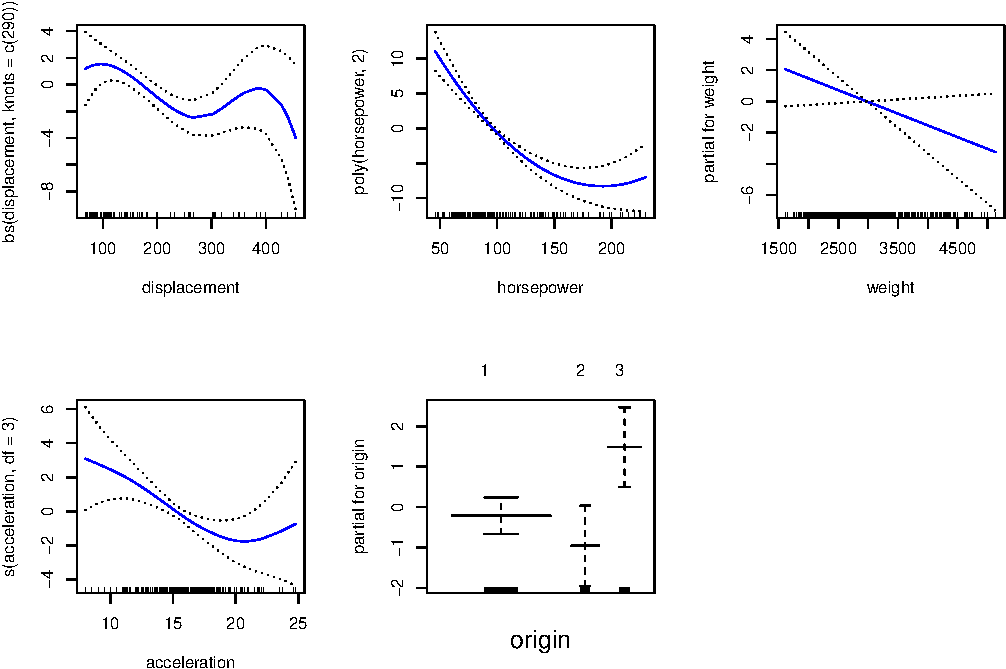
\includegraphics{11Nnet_files/figure-beamer/unnamed-chunk-7-1.pdf}
\end{frame}

\begin{frame}[fragile]
\begin{block}{Boston example using \texttt{keras}}
\protect\hypertarget{boston-example-using-keras}{}
\(~\)

See recommended exercise.
\end{block}
\end{frame}

\begin{frame}{Convolutional neural networks (CNNs)}
\protect\hypertarget{convolutional-neural-networks-cnns}{}
\(~\)

\begin{itemize}
\tightlist
\item
  Motivated by image classification.
\end{itemize}

\(~\)

\begin{itemize}
\tightlist
\item
  Example: the CIFAR-100 dataset
  (\url{https://www.cs.toronto.edu/~kriz/cifar.html}): Images of 100
  categories with 600 images each.
\end{itemize}

\centering

\includegraphics[width=0.4\textwidth,height=\textheight]{cifar10.png}

\flushleft
\scriptsize

(Example from the CIFAR-10 data set with only 10 classes).
\end{frame}

\begin{frame}
\vspace{2mm}

\begin{itemize}
\tightlist
\item
  Idea of CNNs: recognize features and patterns.
\end{itemize}

\vspace{2mm}

\begin{itemize}
\tightlist
\item
  The network identifies \emph{low-level features} (edges, color patched
  etc).
\end{itemize}

\vspace{2mm}

\begin{itemize}
\tightlist
\item
  These low-level features are then combined into \emph{higher-level
  features}.
\end{itemize}

\vspace{2mm}

\begin{itemize}
\tightlist
\item
  Two types of layers: \emph{\textcolor{red}{Convolution layers}} and
  \emph{\textcolor{red}{pooling layers}}.
\end{itemize}
\end{frame}

\begin{frame}
\begin{block}{Convolution layers}
\protect\hypertarget{convolution-layers}{}
\(~\)

\begin{itemize}
\tightlist
\item
  Composed of \emph{filters}.
\end{itemize}

\(~\)

\begin{itemize}
\tightlist
\item
  Example:
\end{itemize}

\[\left[ 
\begin{matrix}
a & b & c \\
d & e & f \\
g & h & i\\
j & k & l \\
\end{matrix}
\right] \qquad \text{Convolved with } \qquad 
\left[ 
\begin{matrix}
\alpha & \beta \\
\gamma & \delta \\
\end{matrix}\right] \] \(\rightarrow\) Convolved image:

\(~\)

\vspace{2cm}

\(~\)

The filter highlights regions in the image that are similar to the
filter itself.
\end{block}
\end{frame}

\begin{frame}
Filtering for vertical or horizontal stripes:

\centering

\includegraphics[width=0.8\textwidth,height=\textheight]{fig107.png}

\scriptsize

(Figure 10.7)
\end{frame}

\begin{frame}
\begin{itemize}
\tightlist
\item
  In \emph{image processing} we would use predefined (fixed) filters.
\end{itemize}

\(~\)

\begin{itemize}
\tightlist
\item
  In CNNs, the idea is that the filters are \emph{learned}.
\end{itemize}

\(~\)

\begin{itemize}
\tightlist
\item
  One filter is applied to each color (red, green, blue), so three
  convolutions are happening in parallel and then immediately summed up.
\end{itemize}

\(~\)

\begin{itemize}
\tightlist
\item
  In addition, we can use \(K\) different filters in a convolution step.
  This produced 3D feature maps (of depth \(K\)).
\end{itemize}

\(~\)

\begin{itemize}
\tightlist
\item
  The convolved image is then also processed with the ReLU activation
  function.
\end{itemize}
\end{frame}

\begin{frame}
\begin{block}{Pooling layers}
\protect\hypertarget{pooling-layers}{}
\(~\)

\begin{itemize}
\tightlist
\item
  Idea: consense/summarize information about the image.
\end{itemize}

\(~\)

\begin{itemize}
\tightlist
\item
  \emph{Max pool}: Use the maximum value in each \(2\times 2\) block.
  \[\left[ 
  \begin{matrix}
  1 & 2 & 5 & 3 \\
  3 & 0 & 1 & 2 \\
  2 & 1 & 3 & 4\\
  1 & 1 & 2 & 0 \\
  \end{matrix}
  \right] \qquad \rightarrow \qquad 
  \left[ 
  \begin{matrix}
  3 & 5 \\
  2 & 4 \\
  \end{matrix}\right] \]
\end{itemize}
\end{block}
\end{frame}

\begin{frame}
In a CNN, we now combine convolution and pooling steps interatively:

\centering

\includegraphics{fig108.png}

\begin{itemize}
\item
  The number of channels after a convolution step is the number of
  filters (\(K\)) that is used in this iteration.
\item
  The dimension of the 2D images after a pooling step is reduced,
  depending on the dimension of the filter (e.g., \(2\times 2\) reduces
  each dimension by a factor of 2).
\item
  In the end, all the dimensions are \emph{flattened} (pixels become
  ordered in 2D).
\item
  The output layer has a \emph{softmax} activation function since the
  aim is classification.
\end{itemize}
\end{frame}

\begin{frame}
\begin{block}{Data augmentation}
\protect\hypertarget{data-augmentation}{}
\(~\)

\begin{itemize}
\tightlist
\item
  Very simple idea: Make the analysis more robust by including
  replicated, but slightly modified pictures of the original data.
\end{itemize}

\(~\)

\begin{itemize}
\tightlist
\item
  Example:
\end{itemize}

\includegraphics[width=0.9\textwidth,height=\textheight]{fig109.png}

\scriptsize Figure 10.9 of James et al. (2021)
\end{block}
\end{frame}

\begin{frame}
\begin{block}{Examples}
\protect\hypertarget{examples}{}
\(~\)

See

\begin{itemize}
\item
  Section 10.3.5 in the book,
\item
  Examples in the recommended exercise 11.
\end{itemize}
\end{block}
\end{frame}

\begin{frame}{Recurrent neural networks (RNNs)}
\protect\hypertarget{recurrent-neural-networks-rnns}{}
\(~\)

\begin{itemize}
\tightlist
\item
  Suitable for data with sequential character.
\end{itemize}

\vspace{2mm}

\begin{itemize}
\tightlist
\item
  Examples: Text documents, time series (temperature, stock prices,
  music, speech,\ldots)
\end{itemize}

\vspace{2mm}

\begin{itemize}
\tightlist
\item
  The input object \(X\) is a sequence.
\end{itemize}

\vspace{2mm}

\begin{itemize}
\tightlist
\item
  In the most simple case, the output \(Y\) is a single value
  (continuous, binary or a category).
\end{itemize}

\vspace{2mm}

\begin{itemize}
\tightlist
\item
  More advanced RNNs are able to map sequences to sequences
  (\emph{Seq2Seq})\footnote{Google Translate uses this technique, for example}
  in language modeling, and much more!
\end{itemize}
\end{frame}

\begin{frame}
\centering

\includegraphics[width=0.8\textwidth,height=\textheight]{fig10_12.png}

\scriptsize Figure 10.12 of James et al. (2021)

\normalsize

\begin{itemize}
\item
  Observed sequence \(X=\{ X_1, \ldots , X_L \}\), where each
  \(X_l^\top=(X_{l1},\ldots, X_{lp})\) is an input vector at point \(l\)
  in the sequence.
\item
  Sequence of hidden layers \(\{ A_1, \ldots, A_L \}\), where each
  \(A_l\) is a layer of \(K\) units
  \(A_l^\top = (A_{l1}, \ldots , A_{lK})\).
\item
  \(A_{lk}\) is determined as \begin{equation}\label{eq:chain}
  A_{lk} = g(w_{k0} + \sum_{j=1}^p w_{kj}X_{lj} + \sum_{s=1}^K u_{ks}A_{l-1,s}) \ ,
  \end{equation}
\end{itemize}

with hidden layer activation function \(g()\) (e.g., ReLU).
\end{frame}

\begin{frame}
\begin{itemize}
\tightlist
\item
  The output is determined as
  \[O_l = \beta_0 + \sum_{k=1}^K\beta_k A_{lk} \ ,\] potentially with a
  sigmoid or softmax output activation for binary or categorical
  outcome.
\end{itemize}

\(~\)

\begin{itemize}
\tightlist
\item
  Note: The weights \(\boldsymbol{W}\), \(\boldsymbol{U}\) and
  \(\boldsymbol{B}\) are the \emph{same} at each point in the sequence.
  This is called \emph{\textcolor{red}{weight sharing}}.
\end{itemize}
\end{frame}

\begin{frame}
\begin{block}{Fitting the weights in an RNN}
\protect\hypertarget{fitting-the-weights-in-an-rnn}{}
\(~\)

\begin{itemize}
\tightlist
\item
  Minimize a \emph{loss function}. In regression problems:
  \[\text{Loss} = (Y- O_L)^2 \ . \]
\end{itemize}

\(~\)

\begin{itemize}
\tightlist
\item
  Only the \emph{last observation} is relevant. How can this be
  meaningful?
\end{itemize}

\(~\)

\begin{itemize}
\tightlist
\item
  Reason: each element \(X_l\) contributes to \(O_L\) via equation (1).
\end{itemize}

\(~\)

\begin{itemize}
\tightlist
\item
  For input sequences \((x_i,y_i)\), we minimize
  \(\sum_{i=1}^n (y_i - o_{iL})^2\).
\end{itemize}

\(~\)

\begin{itemize}
\tightlist
\item
  Note: \(x_i = \{ x_{i1}, \ldots, x_{iL} \}\) is a sequence of
  \emph{vectors}.
\end{itemize}
\end{block}
\end{frame}

\begin{frame}
Why are the outputs \(O_1, \ldots, O_{L-1}\) there at all?

\(~\)

\pause

\textbf{A}:

\begin{itemize}
\item
  They come for free (same weights \(\boldsymbol{B}\)).
\item
  Sometimes, the output is a whole sequence.
\end{itemize}
\end{frame}

\begin{frame}
\begin{block}{Example of an RNN: Time series forecasting}
\protect\hypertarget{example-of-an-rnn-time-series-forecasting}{}
\vspace{2mm}

Trading statistics from New York Stock exchange:

\centering

\includegraphics[width=0.7\textwidth,height=\textheight]{fig10_14.png}

\scriptsize Figure 10.14 of James et al. (2021)
\end{block}
\end{frame}

\begin{frame}
\(~\)

\textbf{Observations: }

\(~\)

\begin{itemize}
\item
  Every day (\(t=1,\ldots, 6051\)) we measure three things, denoted as
  \((v_t, r_t, z_t)\).
\item
  All three series have high \emph{autoc-orrelation}.
\end{itemize}

\(~\)

\(~\)

\textbf{Aim:}

\begin{itemize}
\tightlist
\item
  Predict \(v_t\) from

  \begin{itemize}
  \tightlist
  \item
    \(v_{t-1}\), \(v_{t-2}\), \ldots,
  \item
    \(r_{t-1}\), \(r_{t-2}\), \ldots, and
  \item
    \(z_{t-1}\), \(z_{t-2}\), \ldots{}
  \end{itemize}
\end{itemize}

\(~\)

But, how do we represent this problem in terms of Figure 10.12?
\end{frame}

\begin{frame}
The idea is to extract shorter series up to a \emph{lag} of length
\(L\):

\(~\)

\[X_1 = \left( 
\begin{matrix}
v_{t-L}\\
r_{t-L}\\
z_{t-L}
\end{matrix}
\right), \ 
\quad X_1 = \left( 
\begin{matrix}
v_{t-L+1}\\
r_{t-L+1}\\
z_{t-L+1}
\end{matrix}
\right), 
\quad 
X_1 = \left( 
\begin{matrix}
v_{t-1}\\
r_{t-1}\\
z_{t-1}
\end{matrix}
\right), 
\quad 
Y = v_t\]

\(~\)

\begin{itemize}
\tightlist
\item
  And then continue to formulate the model as indicated in Figure 10.12.
\end{itemize}
\end{frame}

\begin{frame}{When to use deep learning?}
\protect\hypertarget{when-to-use-deep-learning}{}
\(~\)

\begin{itemize}
\tightlist
\item
  We have learned about many new ``fancy'' and trendy methods. But is it
  always worth using the most advanced ones?
\end{itemize}

\(~\)

\begin{itemize}
\tightlist
\item
  Important: Try the simple methods as well. Sometimes they perform
  quite well.
\end{itemize}

\(~\)

\begin{itemize}
\tightlist
\item
  Advantage of e.g.~simple linear regression?
\end{itemize}
\end{frame}

\begin{frame}[fragile]
\begin{block}{Example: The Hitters data set}
\protect\hypertarget{example-the-hitters-data-set}{}
\(~\)

\begin{itemize}
\tightlist
\item
  Remember from Chapter 6: Prediction of \texttt{Salary} for 263
  baseball players.
\end{itemize}

\(~\)

We compare

\vspace{2mm}

\begin{itemize}
\tightlist
\item
  Linear model with 20 parameters.
\item
  Lasso with CV, where 12 variables remain in the model
\item
  A NN with one hidden layer and 64 units. The model has 1049
  parameters.
\end{itemize}
\end{block}
\end{frame}

\begin{frame}
\includegraphics{Table10_2.png} \(~\)

Conclusions?

\begin{itemize}
\tightlist
\item
  \ldots{}
\item
  \ldots{}
\item
  \ldots{}
\end{itemize}
\end{frame}

\begin{frame}
Lots of papers like those, e.g.~in medicine:

\centering

\includegraphics[width=0.8\textwidth,height=\textheight]{ML_logreg1.png}

\(~\)

\includegraphics[width=1\textwidth,height=\textheight]{ML_logreg2.png}

\includegraphics[width=1\textwidth,height=\textheight]{ML_logreg3.png}
\end{frame}

\begin{frame}{References and further reading}
\protect\hypertarget{references-and-further-reading}{}
\begin{itemize}
\tightlist
\item
  \url{https://youtu.be/aircAruvnKk} from 3BLUE1BROWN - 4 videos - using
  the MNIST-data set as the running example
\item
  Look at how the hidden layer behave:
  \url{https://playground.tensorflow.org}
\item
  Friedman, Hastie, and Tibshirani (2001),Chapter 11: Neural Networks
\item
  Efron and Hastie (2016), Chapter 18: Neural Networks and Deep Learning
\item
  Chollet and Allaire (2018)
\item
  Goodfellow, Bengio, and Courville (2016) (used in IT3030)
  \url{https://www.deeplearningbook.org/}
\item
  Explaining backpropagation
  \url{http://neuralnetworksanddeeplearning.com/chap2.html}
\item
  Slides from MA8701 (Thiago Martins)
  \url{https://www.math.ntnu.no/emner/MA8701/2019v/DeepLearning/}
\end{itemize}
\end{frame}

\begin{frame}{Acknowledgements}
\protect\hypertarget{acknowledgements-1}{}
\hypertarget{refs}{}
\begin{CSLReferences}{1}{0}
\leavevmode\vadjust pre{\hypertarget{ref-kerasR}{}}%
Chollet, François, and J. J. Allaire. 2018. \emph{Deep Learning with r}.
Manning Press. \url{https://www.manning.com/books/deep-learning-with-r}.

\leavevmode\vadjust pre{\hypertarget{ref-casi}{}}%
Efron, Bradley, and Trevor Hastie. 2016. \emph{Computer Age Statistical
Inference - Algorithms, Evidence, and Data Science}. Cambridge
University Press.

\leavevmode\vadjust pre{\hypertarget{ref-ESL}{}}%
Friedman, Jerome, Trevor Hastie, and Robert Tibshirani. 2001. \emph{The
Elements of Statistical Learning}. Vol. 1. Springer series in statistics
New York.

\leavevmode\vadjust pre{\hypertarget{ref-goodfellow}{}}%
Goodfellow, Ian, Yoshua Bengio, and Aaron Courville. 2016. \emph{Deep
Learning}. MIT Press.

\leavevmode\vadjust pre{\hypertarget{ref-ISL}{}}%
James, Gareth, Daniela Witten, Trevor Hastie, and Robert Tibshirani.
2021. \emph{An Introduction to Statistical Learning}. 2nd ed. Vol. 112.
Springer.

\end{CSLReferences}
\end{frame}

\end{document}
